\documentclass{beamer}

% \usepackage{beamerthemesplit} // Activate for custom appearance

\title{Remedial Measures Wrap-Up and Transformations-Box Cox}
\author{Frank Wood}
%\date{\today}

\newcommand{\comment}[1]{}
\newcommand{\ponedec}{\mathcal{P}^\downarrow_1}
\newcommand{\pone}{\mathcal{P}_1}
\newcommand{\rank}[1]{\mathrm{RANK}\left[#1\right]}
\newcommand{\E}[1]{\mathrm{E}\left[#1\right]}
\newcommand{\py}{\mathcal{PY}}
\newcommand{\iid}{iid.}
\newcommand{\drawiid}{\stackrel{\text{iid}}{\sim}}
\newcommand{\vect}[1]{\mathbf{#1}}
\newcommand{\indicator}[1]{\text{I}\left[ #1 \right]}
\newcommand{\pdcoag}{PD(d_1,0)-\text{COAG}}
\newcommand{\todo}{\textbf{*TODO*}}
\newcommand{\igram}{\text{$\infty$-gram}}
\newcommand{\Prob}{\text{P}}

\def\mm{sequence memoizer }
\def\MM{SM }

\def\pibf{{\boldsymbol{\pi}}}
\def\kapbf{\boldsymbol{\kappa}}
\def\taubf{\boldsymbol{\tau}}
\def\thebf{\boldsymbol{\theta}}
\def\rhobf{\boldsymbol{\rho}}
\def\phibf{\boldsymbol{\phi}}
\def\pbf{\mathbf{p}}
\def\qbf{\mathbf{q}}
\def\sbf{\mathbf{s}}
\def\tbf{\mathbf{t}}
\def\ybf{\mathbf{y}}
\def\wbf{\mathbf{w}}
\def\xbf{\mathbf{x}}
\def\rbf{\mathbf{r}}
\def\tbf{\mathbf{t}}
\def\kbf{\mathbf{k}}
\def\Xbf{\mathbf{X}}
\def\0bf{\mathbf{0}}
\def\Ibf{\mathbf{I}}
\def\phibf{\mathbf{\phi}}
\def\Phibf{\mathbf{\Phi}}
\def\disteq{{\stackrel{D}{=}}}
\def\EE{{\mathbb{E}}}

\def\phiv{\varphi}
\def\phivbf{\boldsymbol{\varphi}}

\def\Ocal{\mathcal{O}}

\DeclareMathOperator*{\Bet}{Beta} \DeclareMathOperator{\coag}{COAG}
\DeclareMathOperator{\frag}{FRAG} \DeclareMathOperator*{\rnk}{RANK}
\DeclareMathOperator*{\gem}{GEM} \DeclareMathOperator*{\pd}{PD}
\DeclareMathOperator*{\gd}{GDir} \DeclareMathOperator*{\Dir}{Dir}
\DeclareMathOperator*{\Ave}{\mathbb{E}}
\DeclareMathOperator*{\Var}{Var}

\begin{document}

\frame{\titlepage}

%\section[Outline]{}
%\frame{\tableofcontents}
%
%\section{Introduction}
%\subsection{Overview of Topics}
%
%\section{Bayesian Analysis}
%\subsection{Single Parameter Model}
\frame[t] {
 \frametitle{Last Class}
 \begin{itemize}
 \item Graphical procedures for determining appropriateness of
 regression fit\\
 - Normal probability plot
 \item Tests to determine\\
 - Constancy of error variance\\
 - Appropriateness of linear fit
 \item what do we do if we determine(through testing or otherwise)
 that the linear regression fit is not good?
 \end{itemize}
}

\frame[t] {
 \frametitle{Overview of Remedial Measures}
 If simple regression model is not appropriate then there are two
 choices:\\
 1. Abandon simple regression model and develop and use a more
 appropriate model\\
 2. Employ some transformation of the data so that the simple
 regression model is appropriate for the transformed data.
}

\frame[t] {
 \frametitle {Fixes For...}
 \begin{itemize}
 \item Nonlinearity of regression function
 - Transformation(s) (today)
 \item Nonconstancy of error variance
 - Weighted least squares (nice project idea, coming later in class)
 and transformations
 \item Nonindependence of error terms
 - Directly model correlation or use first differences (may skip)
 \item Non-normality of error terms
 - Transformation(s) (today)
 \item Outlying observations
 - Robust regression (another nice project idea)
 \end{itemize}
}

\frame[t] {
 \frametitle{Nonlinearity of regression function}
 Direct approach\\
 \begin{itemize}
 \item Modify regression model by altering the nature of the
 regression function. For instance, a quadratic regression function
 might be used
 \begin{center}
 $E(Y)=\beta_0+\beta_1 X+\beta_2 X^2$
 \end{center}
 \item or an exponential function
 \begin{center}
 $E(Y)=\beta_0 \beta_1^X$
 \end{center}
 \item Such approaches employ a tranformation to (approximately)
 linearize a regression function
 \end{itemize}
}

\frame[t] {
 \frametitle{Quick Questions}
 \begin{itemize}
 \item How would you fit such models?
 \item How does the exponential regression function relate to
 regular linear regression?
 \item Where did the error terms go?
 \end{itemize}
}

\frame[t] {
 \frametitle{Transformations}
 Transformations for nonlinearity relation only\\
 - Appropriate when the distribution of the error terms is
 reasonably close to a normal distribution\\
 - In this situation\\
 1. transformation of X should be attempted;\\
 2. transformation of Y should not be attempted because it will
 materially effect the distribution of the error terms.
}

\frame[t] {
 \frametitle{Prototype Regression Patterns}
\begin{figure}[h!]
   \centering
     \caption{}
     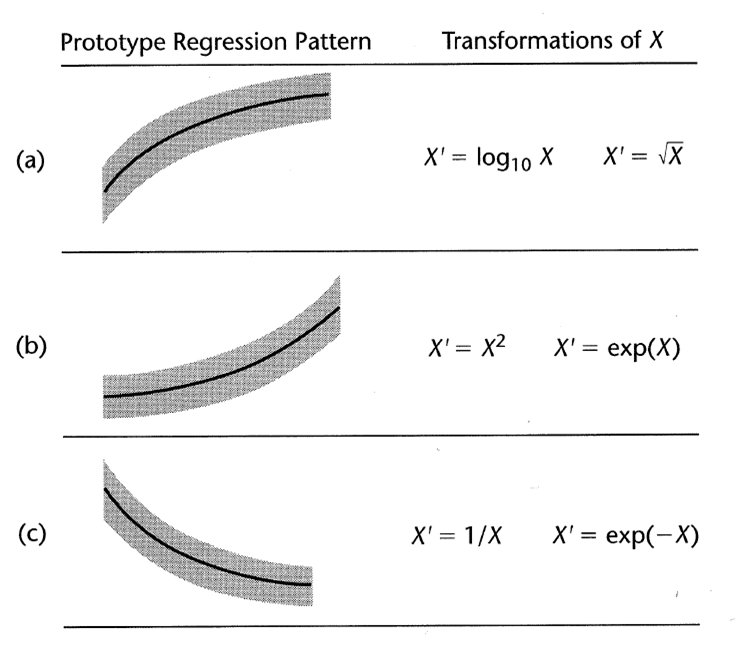
\includegraphics[scale=.4]{8.png}
 \end{figure}
}

\frame[t] {
 \frametitle{Example}
 Experiment\\
 -X: days of training received\\
 -Y: sales performance(score)
}

\frame[t] {
 \frametitle{$X'=\sqrt{X}$}
 \begin{figure}[h!]
   \centering
     \caption{}
     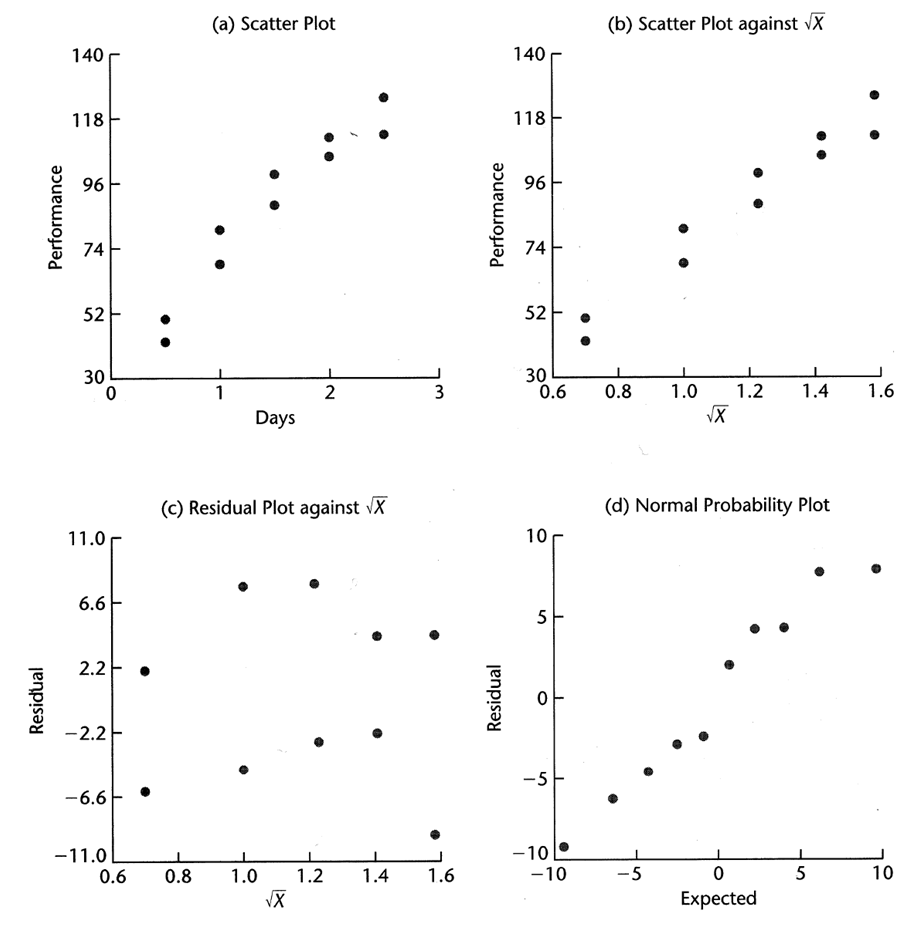
\includegraphics[scale=.4]{10.png}
 \end{figure}

}

\frame[t] {
 \frametitle{Example Data Transformation}
 \begin{figure}[h!]
   \centering
     \caption{}
     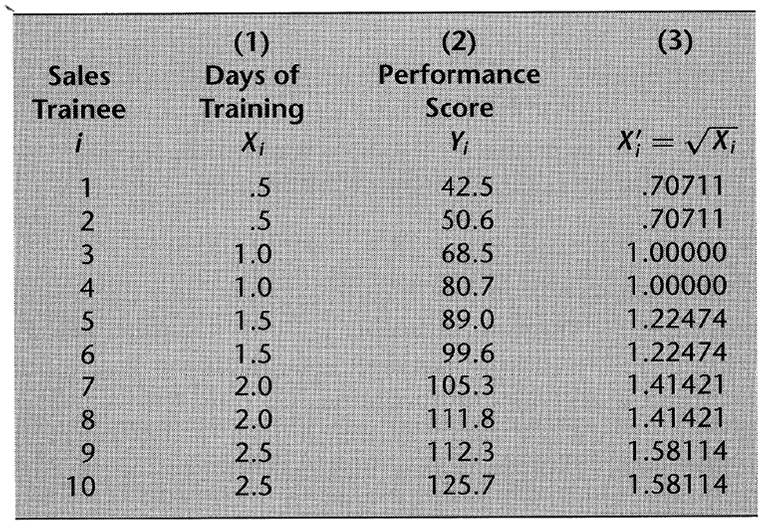
\includegraphics[scale=.4]{11.png}
 \end{figure}
}

\frame[t] {
 \frametitle{Graphical Residual Analysis}
 \begin{figure}[h!]
   \centering
     \caption{}
     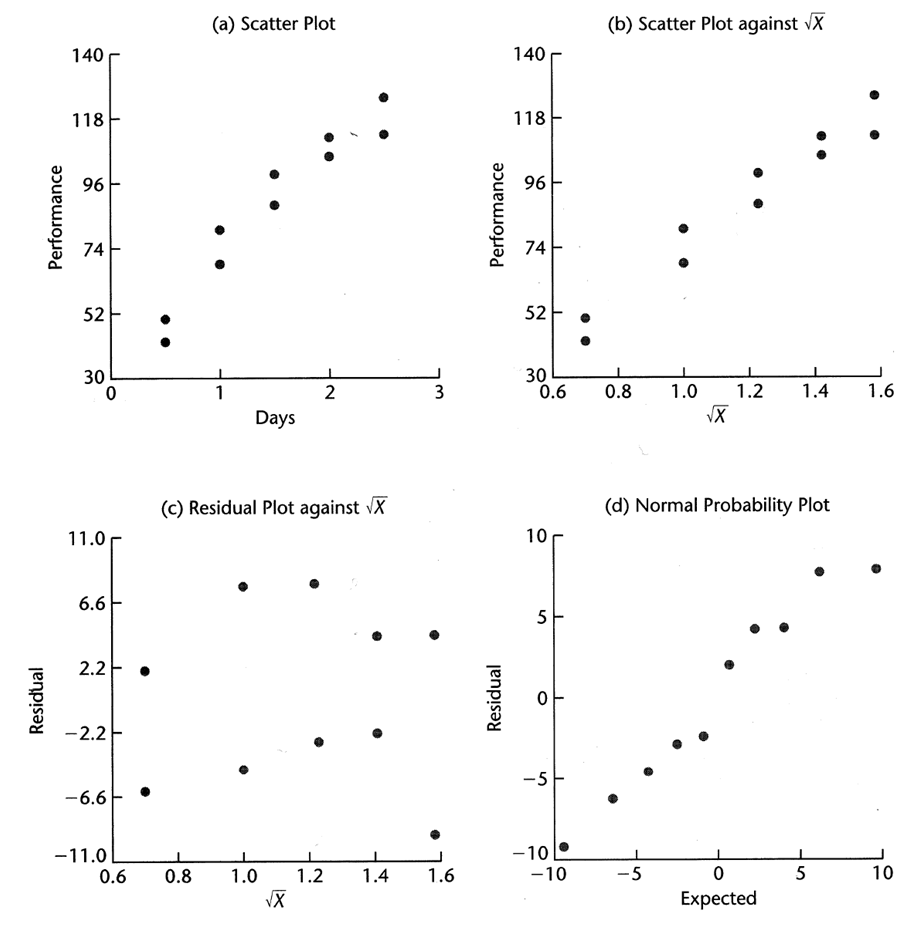
\includegraphics[scale=.4]{12.png}
 \end{figure}
}

%\frame[t] {
 %\frametitle{Matlab}
% Run matlab$\_$demos$\setminus$transform$\_$X.m
%}

\frame[t] {
 \frametitle{Transformations on Y}
 \begin{itemize}
 \item Non-normality and unequal variances of error terms frequently
 appear together
 \item To remedy these in the normal regression model we need a
 transformation on Y
 \item This is because\\
 - Shapes and spreads of distributions of Y need to be changed\\
 - May help linearize a curvilinear regression relation
 \item Can be combined with transformation on X
 \end{itemize}
}

\frame[t] {
 \frametitle{Prototype Regression Patterns and Y Transformations}
 \begin{figure}[h!]
   \centering
     \caption{}
     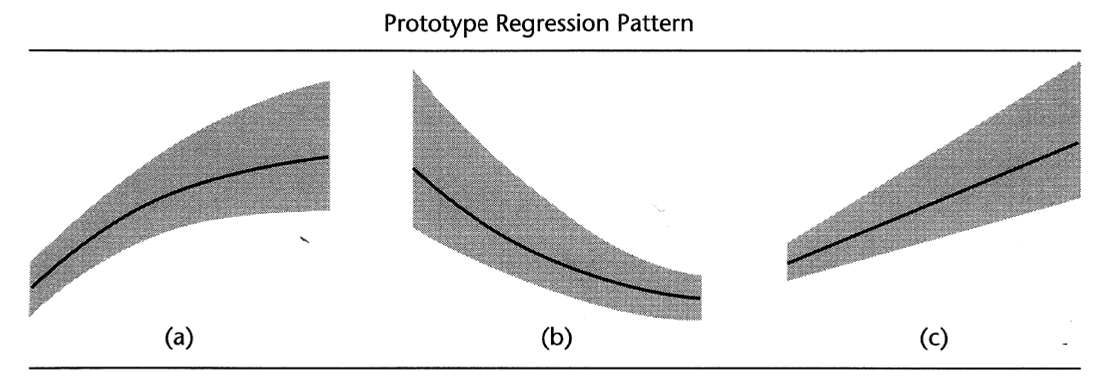
\includegraphics[scale=.4]{15.png}
 \end{figure}
 Transformations on Y:\\
 $y'=\sqrt{Y}$\\
 $y'=log_10 Y$\\
 $y'=1/Y$
}

\frame[t] {
 \frametitle{Example}
 \begin{itemize}
 \item Use of logarithmic transformation of Y to linearize
 regression relations and stabilize error variance
 \item Data on age(X) and plasma level of a polyamine (Y) for a
 portion of the 25 healthy children in a study. Younger children
 exhibit greater variability than older children.
 \end{itemize}
}

\frame[t] {
 \frametitle{Plasma Level vs. Age}
 \begin{figure}[h!]
   \centering
     \caption{}
     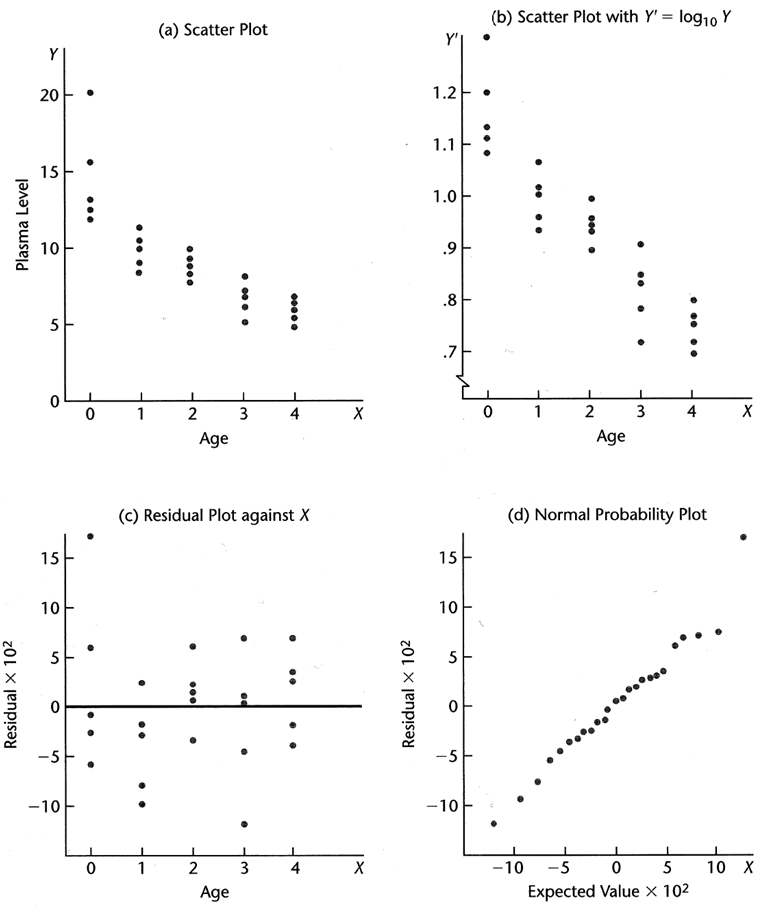
\includegraphics[scale=.4]{17.png}
 \end{figure}
}

\frame[t] {
 \frametitle{Associated Data}
 \begin{figure}[h!]
   \centering
     \caption{}
     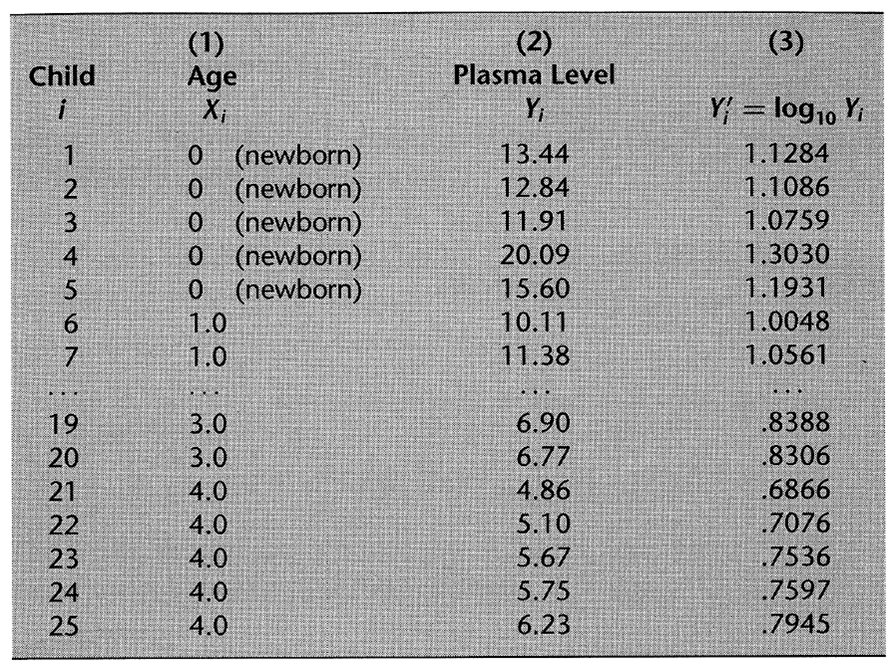
\includegraphics[scale=.4]{18.png}
 \end{figure}
}

\frame[t] {
\begin{itemize}
\item if we fit a simple linear regression line to the log
transformed Y data we obtain:
\begin{center}
$\hat{Y}'=1.135-.1023X$
\end{center}
\item And the coefficient of correlation between the ordered
residuals and their expected values under normality is .981(for
$\alpha=.05$ B.6 in the book shows a critical value of .959)
\item Normality of error terms supported, regression model for
transformed Y data appropriate.
\end{itemize}
}


\frame[t] {
 \frametitle{Box Cox Transforms}
 \begin{itemize}
 \item It can be difficult to graphically determine which
 transformation of Y is most appropriate for correcting\\
 - skewness of the distributions of error terms\\
 - unequal variances\\
 - nonlinearity of the regression function
 \item The Box-Cox procedure automatically identifies a
 transformation from the family of power transformations on Y
 \end{itemize}
}

\frame[t] {
 \frametitle{Box Cox Transforms}
 \begin{itemize}
 \item This family is of the form
 \begin{center}
 $Y'=Y^\lambda$
 \end{center}
 \item Examples include\\
 \begin{center}
 $\lambda=2~~~~Y'=Y^2$\\
 $\lambda=.5~~~~Y'=\sqrt{Y}$\\
 $\lambda=0~~~~Y'=ln Y$ (by definition)\\
 $\lambda=-.5~~~~Y'=\frac{1}{\sqrt{Y}}$\\
 $\lambda=-1~~~~Y'=\frac{1}{Y}$\\
 \end{center}

 \end{itemize}
}

\frame[t] {
 \frametitle{Box Cox Cont.}
 \begin{itemize}
 \item The normal error regression model with the response variable
 a member of the family of power transformations becomes
 \begin{center}
 $Y_i^\lambda=\beta_0+\beta_1 X_i+\epsilon_i$
 \end{center}
 \item This model has an additional parameter that needs to be
 estimated
 \item Maximum likelihood is a way to estimate this parameter
 \end{itemize}
}

\frame[t] {
 \frametitle{Box Cox Maximum Likelihood Estimation}
 \begin{itemize}
 \item Before setting up MLE, the observations are further
 standardized so that the magnitude of the error sum of squares does
 not depend on the value of $\lambda$
 \item The transformation is give by\\
 \begin{center}
 \begin{align*}
 W_i&=K_1(Y_i^\lambda-1)~~~\lambda \neq 0\\
    &=k_2(log_e Y_i)~~~\lambda=0
 \end{align*}
  \end{center}
 where
 \begin{center}
 $K_2=(\prod Y_i)^{1/n}$\\
 $K_1=\frac{1}{\lambda K_2^{\lambda-1}}$
 \end{center}

 \end{itemize}
}

\frame[t] {
 \frametitle{Box Cox Maximum Likelihood Estimation}
 \begin{itemize}
 \item Maximize\\
 %\begin{center}
 $log(L(X,Y,\sigma,\lambda,b_1,b_0))=-\displaystyle\sum_i
 \frac{(W_i-(b_1X_i+b_0))^2}{2\sigma^2}-nlog(\sigma)$\\
 %\end{center}
 w.r.t $\lambda~~\sigma~~b_1~~b_0$
 \item How?\\
 - Take partial derivatives\\
 - Solve\\
 - or... gradient ascent methods
 \end{itemize}
}

\frame[t] {
 \frametitle{Comments on Box Cox}
 \begin{itemize}
 \item The Box-Cox procedure is ordinarily used only to provide a
 guide for selecting a transformation
 \item At time, theoretical or other a priori considerations can be
 utilized to help in choosing an appropriate transformation
 \item It is important to perform residual analysis after the
 transformation to ensure the transformation is appropriate
 \item When transformed models are employed, $b_0$ and $b_2$
 obtained via least squares have the least squares property w.r.t
 the transformed observations not the original ones.
 \end{itemize}
}




\end{document}
